\chapter{Транспортные свойства и особенности кристаллической структуры соединений из группы тетраэдрита"--~теннантита (литературный обзор)} \label{chapt1}

Современное развитие техники предъявляет новые требования к функциональным материалам, задача поиска которых стоит перед наукой. Общепринятый способ получаения термоэлектрических материалов заключается в модифицировании поликристаллических структур допированием атомами, которые повышают электропроводность. Другой способ~--- наноструктурирование материала, который используется для создания низкой, подразумевается стеклоподобной, теплопроводности с высоким значением электропроводности, которая создается за счет проводящего межзеренного пространства. Еще один способ создания термоэлектрических материалов основывается на создании стеклоподоной теплопроводности за счет наличия в кристаллической структуре обособленных комлексов атомов. Одними из таких перспективных функциональных материалов являются соединения из группы тетраэдрита"--~теннантита с обшей структурной формулой (Cu\textsuperscript{+},Fe,Ag,Zn)\textsubscript{10}(Cu\textsuperscript{2+})\textsubscript{2}(As,Sb)\textsubscript{4}(S,Se)\textsubscript{13}.

Соединения группы тетраэдрита"--~теннантита так же называют блеклыми рудами или сульфосолями. Кристаллическая структура соединений группы тетраэдрита"--~теннантита описывается кубической плотноупакованной структурой с расположением катионов в лавесовских полиэдрах. Такая структура близка с сфалеритовой структуре, но с параметром ячейки вдвое большим, чем у сфалерита. Своё название она  получили благодаря тусклому блеску на изломе. В минералогии эти минералы уже более чем 250 лет используются как индикаторы условий рудообразования.

Соединения ряда тетраэдрит--теннантит согласно принятой классификации в минералогии\cite{Molo2008} относят к большой семье из подтипа сульфосолей класса халькогенидов, выделенных по химическим особенностям.  
Понятие сульфосолей включает в себя широкий класс соединений (имеются ввиду минералы) содержащих трёхвалентные атомы As, Sb, Bi и за редким исключением четырехвалентного Te. 
Подразумевается, что катионы As\textsuperscript{3+}, Sb\textsuperscript{3+}, Bi\textsuperscript{3+} и Te\textsuperscript{4+} связаны с катионом или катионами Me. 
Причем анион  S\textsuperscript{2-} может быть заменен на Se\textsuperscript{2-} или Te\textsuperscript{2-}. Таким образом, общая зарядовая формула сульфосолей имеет следующий вид:

\begin{equation}
  \label{eq:equation1}
  (Me^+,Me^{'2+},etc.)_{x}[(Bi, Sb,As)^{3+}, Te^{4+}]_{y}[(S,Se,Te)^{(2-)}]_{z}.
\end{equation}

Важно отметить, что отличительной особенностью сульфосолей является электронное взаимодействие между катионами, например As\textsuperscript{3+}, Sb\textsuperscript{3+}, Bi\textsuperscript{3+}, ввиду их ассиметричного расположения. Такая отличительная особенность структуры выделяет соединения с общей структурной формулой  \eqref{eq:equation1} в особую группу в классе халькогенидов. Данная классификация была введена по аналогии с существующей классификацией оксидов, как для (As\textsuperscript{3+}O\textsubscript{3})\textsuperscript{3$-$} или (As\textsuperscript{5+}O\textsubscript{4})\textsuperscript{3$-$}\cite{Nowacki1969}.

В общем случае соединения ряда тетраэдрит--теннантит описываются структурной формулой: 

\begin{equation}
  \label{eq:equation2}
      \begin{multlined}
      (Cu^{1+},Ag,Tl,Au)_{10}(Zn,Fe,Cu^{2+},Hg,Cd,Pb,Mn,Ni,Co,Sn)_{2}\times \\
      \times(As,Sb,Bi,Te,Ge,In)_{4}(S,Se)_{13}. 
      \end{multlined}
\end{equation}
\newpage

%\newpage
%============================================================================================================================

\section{Структурные особенности соединений теннантита и тэтраэдрита и их связь с транспортными свойствами} \label{sect1_1}

 Структура тетраэдрита впервые была описана Паулингом и Нейманом  \cite{Pauling1934} и уточнена в работах \cite{Wuensch1963,Wuensch1964,Belov1969,Kaplunnik1980}.
 В соврмененной литературе встречается два вида структурной формулы Cu(I)\textsubscript{6}Cu(II)\textsubscript{6}[(As,Sb)S\textsubscript{3}]S\textsubscript{4}\cite{Johnson1986} и Cu$_{10-x}^{+}$Cu$_{2+x}^{2+}$(As,Sb)$_{4}^{3+}$S$_{13}^{2-}$ \cite{Friese2008,makovicky2005crystal,Foit2001} (группа симметрии I$\overline{\! 4}$3m).
Данные соединения являются наиболее хорошо изученными и широко представленны в литературе. Структуру соединений теннантита~--тэтраэдрита представляет собой тэтраэдрические комплексы  CuVI\textsubscript{4}, где VI = S, Se, ориентированные в пространстве в одну сторону (Рис. \ref{img:figure1}а). Такое упорядочение тэтраэдрических комплексов создает пустоты между ними и эти пустоты имеют форму усеченных тэтраэдров (<<лавесовские поллиэдры>>). <<Лавесовские поллиэдры>> изображенны на рисунке~\ref{img:figure1}б). В полученных усеченных тэтраэдрах помещаются по шесть атомов меди (Рис. \ref{img:figure1}в), каждый из которых окружен тремя атомами серы\cite{Makovicky_2006}. Величина параметра элементарной ячейки изменяется от 10.16 до 10.33, ввиду ограниченного изоморфизма.

\begin{figure}[pt!]
  \begin{minipage}[ht]{0.99\linewidth}\centering
    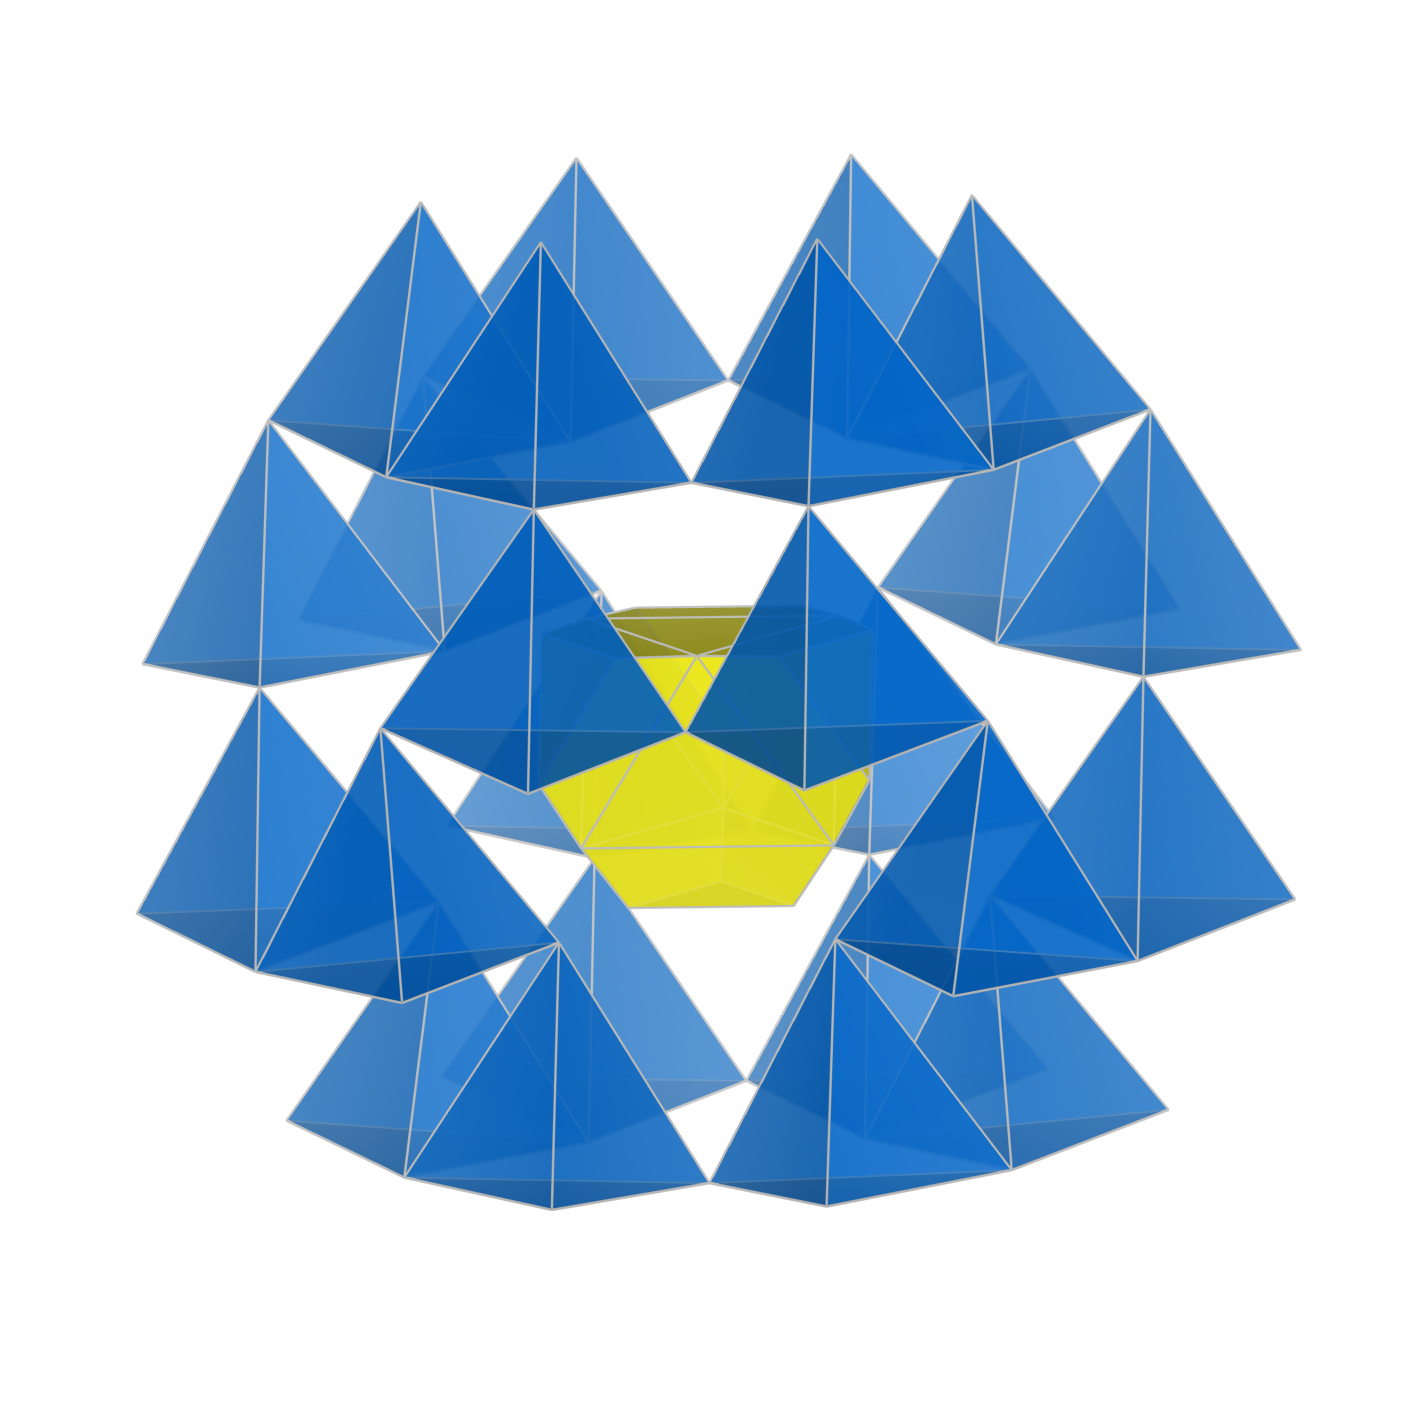
\includegraphics[width=0.6\linewidth]{2_cu12as4s13_crys_st_b} \\ а)
  \end{minipage}
  \vfill
  \begin{minipage}[ht]{0.99\linewidth}\centering
    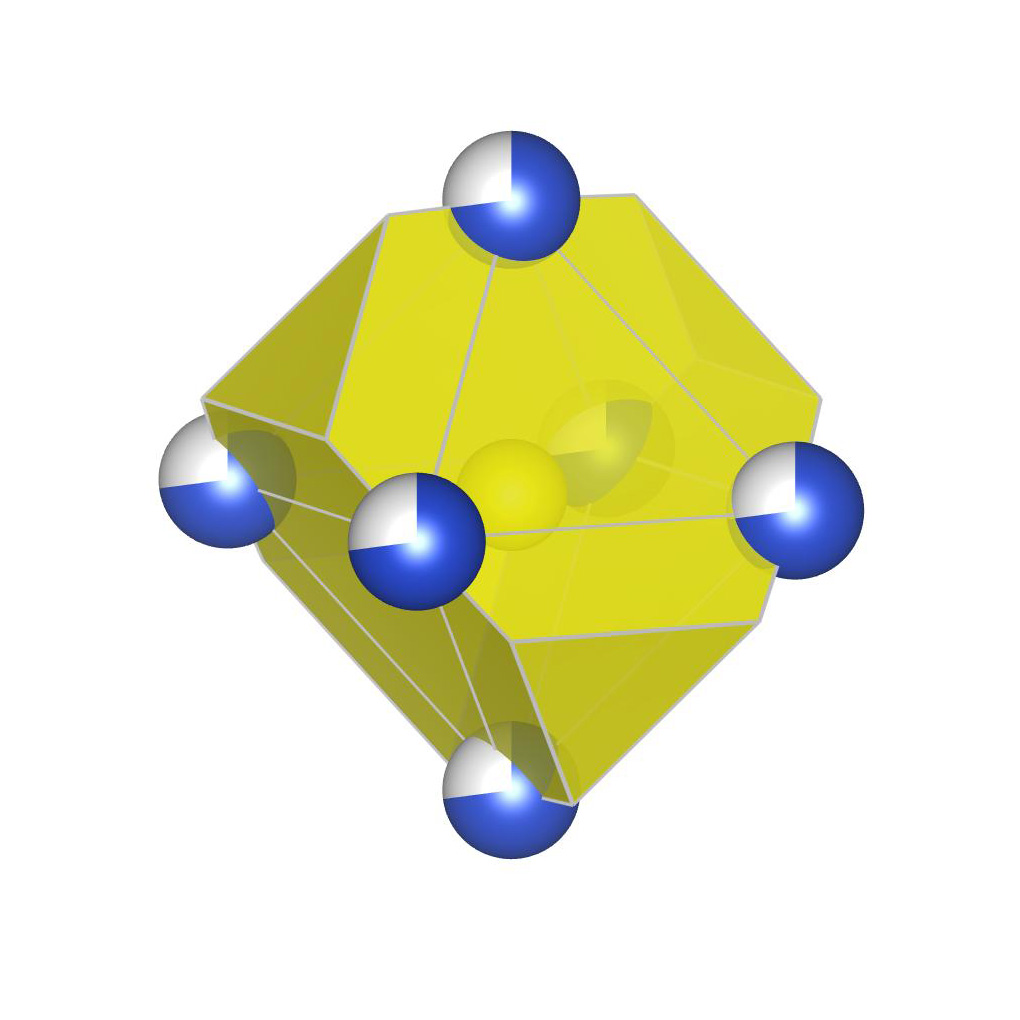
\includegraphics[width=0.6\linewidth]{3_cu12as4s13_crys_st_d} \\ б)
  \end{minipage}

      \caption[Кристаллическая структура халькогенида на примере синтетического теннантита Cu\textsubscript{12}As\textsubscript{4}S\textsubscript{13}]{Кристаллическая структура халькогенида на примере синтетического теннантита Cu\textsubscript{12}As\textsubscript{4}S\textsubscript{13}}
    \label{img:figure1}
\end{figure}

Структура соединений теннантит и тэтраэдрит является близкой к  подобным структурам сфалерита или халькопирита\cite{Pauling1934}. 
Если увеличить структуру сфалерита ZnS вдвое по ребру, то элементарная ячейка будет содержать в восемь раз больше атомов: 32 катиона Zn\textsuperscript{2+} и 32 аниона S\textsuperscript{2+}. И, заменяя часть металлических катионов Zn\textsuperscript{2+} катионами полуметтала X\textsuperscript{3+} и оставляя часть катионов одновалентными X\textsuperscript{+}, получается состав A$^{+}_{24}$X$^{3+}_{8}$S$^{2-}_{32}$. Удаление восьми анионов S\textsuperscript{2-} создает характерные для тэтраэдрита комплексы полуметаллов [X$^{3+}$S$^{2-}_{3}$]. Получившиеся дефекты образуют форму тетраэдров, соответствующую пустым октантам сфалеритовой ячейки. В месте восьми анионов S\textsuperscript{2-} находятся атомы полуметалла  X\textsuperscript{3+}, которые вносят  неподеленные электронные пары. Таким образом, получается, что половина всех ионов A\textsuperscript{+} вблизи тэтраэдров находится без полноценного окружения, координация по анионам S\textsuperscript{2-} равна 2 и координация полуметаллов понижена до трех. Другая половина ионов A\textsuperscript{+} обладает четверной координацией, которая осталась как и у сфалерита. Далее вводится допольнительный анион S\textsuperscript{2-} в центр из двух пустых тетраэдров обратной ориентации, в те места, где находятся неподеленные электронны пары. Введение дополнительного аниона повышает S\textsuperscript{2-}  координацию половины атомов A\textsuperscript{+} до трех. После введения 2S\textsuperscript{2-} необходимо скомпенсировать заряд катионной части на четыре единицы, для чего четыре трехкоординированных катиона A\textsuperscript{+} заменяются на A\textsuperscript{2+}. Получается, что общий состав тэтраэдрита может быть выражен 

\begin{equation}
  \label{eq:equation3}
  A^+_{20}A^{2+}_4[X^{3+}S^{2-}_{3}]^{3-}_{8}S_2.
\end{equation}



В литературе широко обсуждаются возможные методы построения структуры тэтраэдрита. Авторы \cite{Koch_1981} рассматривают стуктуру тэтраэдритов на основе  кубически инвариантного комплека  \textit{W*}, который заполнен дополнительными атомами. Этот комплекс находится  около идеальных тетраэдров с общими общими вершинами с комплексом \textit{W*}. 
Авторы статьи детально обсуждают соединия теннантит и тэтраэдрит с точки зрения гомогенной или негомогенной структур в контексте W*(4t\textsubscript{c}) и (F$^{''}_{2}$-I(4t)) решеток. 
Если рассматривается структура W*, то возможная маскимальная симметричная группа для это структуры Im3m. В этом случае вершины располагаются в позиции 24(h) xx0 с $x = \frac{1}{4}\sqrt{2} = 0.3536$ и центры этих вершин будут располагаться в 12(d) $\frac{1}{4}\frac{1}{2}0$. 
В настоящее время таких структур не найдено, что оставляет открытым вопрос расположения атомов в элементарной ячейке тэтраэдрита. 
Так же известно, значание  z в позиции 24(g) xxz для силикатных структур лежит в диапазоне 0.025~$<$~z~$<$~0.085, в то время как этот же параметр для соедининений с структурой тэтраэдрита лежит в диапазоне 0.135~$<$~z~$<$~0.165.
Исходя из описанного выше, авторы приходят к мнению, что соединения с структурой I$\overline{\!4}$3m могут быть описаны двумя разными гомогенными решетками W*(4t\textsubscript{c}) и (F$^{''}_{2}-$I(4t)).


Авторами работы \cite{Johnson1986} рассмотрено 1271 образцов натурального тэтраэдрита и 295 синтетических образов . Данная работа проведена с целью изучения механизмов замещения элементов Ag, Fe, Zn, Hg, Cd, As, Te, Bi в структуре тэтраэдрита. Исследование показало, что на стркутурную формулу могут приходится от четырех до десяти атомов Cu,  до четырех атомов Ag и не более двух атомов Fe, Zn, Hg. Возможно полное замещение между атомами As и Sb при неизменном составе атомов S в элементарной ячейке. 
По данным авторов описать замещение атомами Pb, Bi и Cd не было возможным ввиду малого количества данных. Структуры с замещенными атомами Co, Ni, Mn и Au не обнаружены. Предложена общая фомула (Cu,Ag)\textsubscript{6}Cu\textsubscript{4}(Fe,Zn,Cu,Hg,Cd)\textsubscript{2}(As,Sb,Bi,Te)\textsubscript{4}(S,Se)\textsubscript{13}. Размер элементарной ячейкаи возрастает с увеличением атомного номера допируемых элементов за исключением тэтраэдритов содержащих Ag. Атомы Ag и As обладают низкой тенденцией к взаимодействию, что подтверждается графиками замещения для Fe от As, Zn от Ag, Hg от Cu. Для объяснения этих механизмов используется модель предложенная Джонсоном \cite{johnson1983brillouin}. Эта модель заключается в анализировании свободных электронов в структуре. Анализ показывает, что структура предсказывает наличие соединений с структурыми формулами  Cu\textsubscript{14}Sb\textsubscript{4}S\textsubscript{13}~--- Cu\textsubscript{12}Sb\textsubscript{4.67}S\textsubscript{13}.

Этими же авторами \cite{Johnson1988} чуть позже обсуждается кристалохимия тетраэдритов и предлагается общая формула \textsuperscript{IV}M(I)\textsubscript{6}\textsuperscript{III}M(II)\textsubscript{6}[\textsuperscript{III}X\textsuperscript{IV}Y\textsubscript{3}]\textsuperscript{VI}Z\textsubscript{4} (M(1) $=$ Cu, Fe, Zn, Mn, Hg, Cd; M(2) $=$ Cu, Ag; X $=$ Sb, As, Bi, Te; Y и Z $=$ S,Se)  для описание структуры тэтраэдрита. Эта структура вводится по аналогии с содалитовой структурой с соединенными тэтраэдрами M(1)Y\textsubscript{4}, которые содержат октаэдры ZM(2)\textsubscript{6}. И авторы предлагают описывать известные экспериментальные данные о структуре тэтраэдритов через вращение тэтраэдров M(1)Y\textsubscript{4} вокруг оси четвертого порядка $\overline{\!4}$. Вращение этих тэтраэдров приводит к вращению всей решетки и это приводит к увеличение связей между M(1)--Y и X--Y, но при этом приводит к уменьшению связи ввиду увеличивания длинны ребра решетки. Искажение решетки тэтраэдра обуславливается влиянием изменения длинны связи M(1)--Y и более сильным влиянием от изменения связи X--Y. Так же отмечается влияние температуры и давления на кристаллографические особенности соединений. В заключении работы авторы делают вывод, что предложенная модель имеет ограничения при построении диаграммы P--T--X и дальнейшие исследования необходимы.

Вариации строения кристаллической структуры и полиморфизм в системе Cu--Sb--S при температуре ниже 400\textsuperscript{$\circ$}С обсуждается в работе \cite{Tatsuka_1977}. Основной результат работы заключается том, что тэтраэдрит стабилен при температуре 95\textsuperscript{$\circ$}С с структурной формулой Cu\textsubscript{12+x}Sb\textsubscript{4+y}S\textsubscript{13}, где 0.11~$\leqslant$~X~$\leqslant$~1.77 и 0.03~$\leqslant$~Y~$\leqslant$~0.3. В работе установлено, что ниже 95\textsuperscript{$\circ$}С соединение тэтраэдрита образует две несмешиваемых фазы, которые описываются структурой тэтраэдрита. Образование фаз быстрое и обратимое. Исследования структуры получившихся фаз показывают, что различие структуры двух фаз заключается в особенностях распеределений позиций меди. Трансформация из одной фазы в другую происходит даже при добавлении лишнего атома меди или серы, в том числе и при комнатной температуре. Отмечается, что при комнатной температуре могут находиться фазы с структурными формулуми Cu\textsubscript{12}Sb\textsubscript{4}S\textsubscript{13} и Cu\textsubscript{14}Sb\textsubscript{4}S\textsubscript{13}. Две эти фазы образуются на основе Cu\textsubscript{3}Sb\textsubscript{0,99}S\textsubscript{3} с параметром ячейки a~$=$~20.848~$\pm$~0.006~$\angstrom$ и имеют название псевдотэтраэдрит. Фаза псевтэтраэдрита стабильна до 350\textsuperscript{$\circ$}С и при более высокой температуре трансформируется в фазы тэтраэдрита. Выше температуры 361\textsuperscript{$\circ$}С так же появляется высокотемпературная фаза Cu\textsubscript{3}SbS\textsubscript{3}. Превращение из фазы Cu\textsubscript{12}Sb\textsubscript{4}S\textsubscript{13} в Cu\textsubscript{14}Sb\textsubscript{4}S\textsubscript{13} и обратно объясняется мобильностью атомов меди в структуре.

Система Cu--As--S исследовалась на особенности формирования фаз методами дифференциального термического анализа и методами рентгенофазового анализа в работе \cite{Kurz_1989}. Установлено наличие квазибинарных соединений Cu\textsubscript{2}S--As, As--Cu\textsubscript{3}AsS\textsubscript{3}, Cu\textsubscript{3}S--Cu\textsubscript{2}S и Cu\textsubscript{2}S--As\textsubscript{2}S\textsubscript{3}. Обнаружено два близких соединения Cu\textsubscript{6}As\textsubscript{4}S\textsubscript{9} и Cu\textsubscript{4}As\textsubscript{2}S\textsubscript{5}. Данные соединения и Cu\textsubscript{24}As\textsubscript{12}S\textsubscript{31} относятся к производной от сфалеритовой структуре и находятся в области гомогенности соединения Cu\textsubscript{4}As\textsubscript{2}S\textsubscript{5} на фазовой диаграмме для системы  Cu--As--S. Отмечается наличие двух модификаций для соединения Cu\textsubscript{3}AsS\textsubscript{3}, низкотемпературная фаза которого известна как теннантит. Высокотемпературная фаза получается закалкой. Некоторые данные показывают, что соединения Cu\textsubscript{5}AsS\textsubscript{4} подобны минералу стэфаниту Ag\textsubscript{5}SbS\textsubscript{4}. Соединения получены спеканием в кварцевых ампулах в вакууме. Часть структурных исследований была проведена на монокристальном дифрактометре Enraf--Nonius CAD 4. В работе детально описываются особенности получения описанных выше фаз.

В статье \cite{Makovicky1995} обсуждается полиморфная фаза Cu\textsubscript{3}SbS\textsubscript{3}. Автором предложена модель  структуры в триклинной сингонии (группа симметрии P2\textsubscript{1}/c). Параметры ячейки a~$=$~7.814(1)~$\angstrom$, b~$=$~10.242(1)~$\angstrom$, c~$=$~13.273(1)~$\angstrom$, $\beta$~$=$~90.29(1)\textsuperscript{$\circ$} c Z~$=$~8. Кристаллическая решетка описывается через деформированную (11$\overline{\!2}$2)\textsubscript{hcp} двойником hcp ряд. Атом Sb находится в треугольной пирамидальной координации в окружении призм, созданных вследствии двоникования из-за ряда атомов~S. Длинна связи Sb--S лежит в диапазоне от 2.26 до 2.47~$\angstrom$. Большинство атомов в позии Cu обладают тройной координацией с длинной связи для Cu--S в диапазоне от 2.26 до 2.31~$\angstrom$. Позиция Cu4 облададает тройной или четверной координацией с длинной связи для Cu--S в диапазоне от 2.40 до 2.46~$\angstrom$. Отмечается, что P2\textsubscript{1}/c--скиннерит является низкотемпературной модификацией Cu\textsubscript{3}SbS\textsubscript{3}. Разница в особенностях расположения атомов меди в структурах P2\textsubscript{1}/c--скиннерит и P2\textsubscript{1}2\textsubscript{1}2\textsubscript{1}/c--виттиханит связывается с разлизным размером полиэдров Sb и Bi соответсвенно. Данные результаты получены из кристалло-химических представлений. 

Авторами \cite{Pfitzner1998a} продолжена классификация фаз соединения Cu\textsubscript{3}SbS\textsubscript{3}. Определена кристаллическая структура $\alpha$--Cu\textsubscript{3}SbS\textsubscript{3} при 493 К и 403 К методами монокристальной дифрактометрии. Высокотемпературная фаза, которая стабильна при температурах выше 394~К, кристализуется в орторомбическую систему: параметры ячейки a~$=$~7.808(1)~$\angstrom$, b~$=$~10.252(2)~$\angstrom$, c~$=$~6.587(2)~$\angstrom$,  c Z~$=$~4, группа симметрии P\textsubscript{nma} (номер 62). Для данного соединения определено распределение атомов меди в тэтраэдре [SbS\textsubscript{3}]\textsuperscript{3-}. Величина отклонения атомов меди определена методом негармоничного развития Грама--Чарля и при условии возможности частичной мобильности атомов. Атомы меди располагаются между пятью позициями с тройной или четверной координацией и пустых октаэдров S\textsubscript{6}. Определена кристаллическая структура $\gamma$--Cu\textsubscript{3}SbS\textsubscript{3}, который стабилен ниже 264~К, методами порошковой дифрактометрии при температуре 223~K. Низкотемпературная фаза кристализуется в орторомбическую систему: параметры ячейки a~$=$~7.884(1)~$\angstrom$, b~$=$~10.221(1)~$\angstrom$, c~$=$~6.624(1)~$\angstrom$,  c Z~$=$~4, группа симметрии P2\textsubscript{1}2\textsubscript{1}2\textsubscript{1} (номер 19). Исследованные образцы получены спеканием в эвакуированных ампулах из соединений Cu\textsubscript{2}S и Sb\textsubscript{2}S\textsubscript{3} при температуре 853~К. Методика получения описана в работе \cite{Pfitzner_1994}. Отмечается, что структура высокотемпературной фазы определена на образце,  который использовался для определения стуктуры фазы $\beta$--Cu\textsubscript{3}SbS\textsubscript{3}. Обработка данных с монокристального эксперимента проводилась в JANA96, порошкового~---~в FULLPROF. Авторы отмечают, что структура для $\gamma$--Cu\textsubscript{3}SbS\textsubscript{3} получена методом Ритвельда с начальной структурой Cu\textsubscript{3}BiS\textsubscript{3}. Размер параметра кристаллической решетки для Cu\textsubscript{12}Sb\textsubscript{4}S\textsubscript{13} при температуре 223~К брался для определения особенностей структуры Cu\textsubscript{12+x}Sb\textsubscript{4}S\textsubscript{13}. Далее авторы проводят рассуждения о возможных вариантах расположения атомов меди в структуре, основываясь на  функции распределения электронной плотности. Атомы меди в позиции Cu(1) и Cu(2) находятся вне октаэдров S\textsubscript{6}. Атом меди в позиции Cu(3) находится на гранях октаэдра  S\textsubscript{6}. Отмечается, что расстояние между атомами в позиции Cu(1) и Cu(2) составляет 2.099(9)~$\angstrom$. Расстояние между  Cu(1) и Cu(3)  составляет 1.266(9)~$\angstrom$, а расстояние между  Cu(2) и Cu(3)  составляет 1.93(1)~$\angstrom$. Полученные расстояния говорят о возможном нахождении атомов меди во всех трех позициях Cu(1), Cu(2) и Cu(3). Так же авторы замечают, что структура Cu\textsubscript{3}SbS\textsubscript{3} не может быть описана в одной из моноклинных структур. Высокотемпературная модификация имеет разориентировку как минимум вокруг 5 различных позиций. Так же авторы добавляют, что уменьшение расстояние между атомами меди, необходимое для возникновения связи d\textsuperscript{10}--d\textsuperscript{10} оболочек с помощью введения дополнительного атома меди и аниона, может привести к появления сверхрешетки, но дальнейших данных по этому предположению в статье нет.


В работе \cite{Makovicky2005} представленно первое исследование структуры монокристаллического образца минерала теннантит. Формула теннантита по результатом исследования авторов является Cu\textsubscript{12.5}As\textsubscript{0.98}As\textsubscript{0.02}S\textsubscript{13}. Исследование проведено на образце с линейными размерами 108 на 72 на 54 мкм при комнатной температуре и Mo K\textsubscript{$\alpha$} излучении на дифрактометре Bruker SMART CCD. Расстояние между кристаллом и детектором было 3.85 см. Параметры ячейки определены по 1068 рефлексам( I~$>$~8$\sigma$\textsubscript{I}) с помощью программного обеспечения SMART и SAINT. Образец проиндицирован в кубической сингонии I$\overline{\!4}$3m с размером ребра кристаллической ячейки 10.1756(9)~$\angstrom$ c R--фактором 0.072. Авторы отмечают, что основная часть позиций атомов полностью заселена и являлась фиксированной при дальнейшем уточнении структуры. Обнаружено, что позиции меди Cu2A и Cu2B не полностью заселены и установлена корелляция между фактором смещения и заселенностью атомов в этих позициях. Между двумя атомами в позиции Cu2B находится один атом в позиции Cu2A, такое расположение образует ярко выраженные эллипсоиды, рассположенные вдоль линии соединяющей Cu2A и Cu2B.  По мнению авторов, такое расположение атомов подтверждает возможность статистического распределения и возможность движения атомов меди  по этим позициям. Заселенность позиций атомов Cu2A и Cu2B составляет 75 и 17~\% соответветсвенно. Таким образом, получается, что почти в каждой позиции Cu2A находится атом меди. Также данные структурного и химического анализа позывают, что могут существовать ситуации, при которых два атома меди будут находится в позиции  Cu2B. Так же авторы отмечают, что проводили уточнение структуры в группы симметрии P1 и утроенной элементарной ячейки и получили тот же результат, что и при уточнении в кубической симметрии. Рассуждения о частичной заселенности показыват, что в структуре не может находится вакантных позиций в лавесовском полиэдре. В заключении авторы отмечают, что отсутсвие двухвалентных атомов в образце, приводит к возникновению особенностей распределения меди.
 


В работе \cite{Nasonova2016} исследована структура низкотемпературной фазы синтетического тэтраэдрита Cu\textsubscript{12}Sb\textsubscript{4}S\textsubscript{13}. Структура соединения получена методами порошкового рентгенофазового анализа в диапазоне температур от 10 до 293 К. Установлено, что при температуре около 90 К происходит фазовый переход типа металл--полупроводник,  смещение атома серы вдоль поверхности октаэдра Cu\textsubscript{6} и сдвиг атома меди вдоль треугольника S\textsubscript{3} связаны с двумя независимыми позициями атомов серы и резким увеличением расстояния между Cu--Sb. Отмечается, что фазовый переход значительно влияет на транспортные свойства соединения: зарегистрировано резкое возрастание электрического сопротивления. Предположение о предсказании сверхструктуры не подверждено \cite{Tanaka2015}.
По мнению авторов, низкая теплопроводность является следствием наличия квазилокализованных атомов меди, которые приводят к размягчению кристаллической решетки с повышением температуры. 
Исследуемые образцы синтетического тэтраэдрита были получены стандартным ампульным методом в стехиометрическом соотношении 12:4:13 в кварцевых ампулах под давлением 2$\times$10\textsuperscript{-2}~Торр. Ампулы нагревались до 973~К и отжигались в течении трех часов при этой температуре, после медленно охлаждались до 823~К в течении 30 часов и после остывали при выключенной печи до комнатной температуры. Полученные спёки перетерались в агатовой ступке и были спресованны в таблетки при давлении 80--100~бар при комнатной температуре. Полученные таблетки отжигались в вакуумированных ампулах при 773~К в течении 25~часов. Структурные исследования были проведены на канале ID22 Европейского синхротронного источника с энергией $\lambda$~=~0.41066~$\angstrom$ и с шагом 10~К в диапазоне температур от 10 до 150~К и с шагом 15~К в дипазоне температур от 150 до 240~К. Авторы отмечают, что все позиции атомов серы в соединениях Cu\textsubscript{12}Sb\textsubscript{4}S\textsubscript{13} и Cu\textsubscript{12}Sb\textsubscript{4}S\textsubscript{12.8} полностью заселены за исключением позиции Cu(2). Для этих соединений установлены различные коэфициенты атомарных смещений 0.0102(4) и 0.0125(3) для позиции атома S(1), 0.016(2) и 0.019(2) для позиций атома S(2) и размер ребра элементаной ячейки 10.33051(2) и 10.33344(1)~$\angstrom$ соответсвенно для Cu\textsubscript{12}Sb\textsubscript{4}S\textsubscript{13} и Cu\textsubscript{12}Sb\textsubscript{4}S\textsubscript{12.8}. Ввиду близкого расположения позиций атомов Cu(2), для уточнения структуры при низких температурх, взята структура Cu\textsubscript{12}Sb\textsubscript{4}S\textsubscript{13}  при комнатной температуре. До фазового перехода кристаллическая ячейка уменьшаяется, но после зависимость размера кристаллической ячейки перестает уменьшатся и показывает локальный максимум при 40~К. Этот фазый переход вызван изменением положения атомов в позиции Cu(2). Так, максимальное и минимальное расстояние между позициями атома Cu(2) изменяется в три раза, а максимальное расстояния между позициями атомов Cu(2) и Sb(1) возникает при температуре соответсвующей локальному максимуму размера кристаллической ячейки при 40~К. Так же, ниже температуры фазового перехода возникает волна зарядовой плостности или упорядочение зарядов Cu\textsuperscript{$+$}Cu\textsuperscript{$2+$} на атомах меди за счет изменения позиций атомов меди Cu(2). Авторами исследованы траспортные свойства полученных соединений. Из полученных данных авторами была найдена характеристическая температура Дебая, которая возникает ввиду наличия квазилокализованных фононных мод в кристаллической решетке. Авторы отмечают, что полученные ими данные для характеристических температур Эйнштейна отличаются от опубликованных в литературе данных\cite{Lara-Curzio2014}. 

В работе \cite{Friese2008} проведено исследование синтетичского теннантита и тэтраэдрита, доппированного железом при температурах 25 и 250\textsuperscript{$\circ$}С. Исследованные соединения обладают структурной формулой Cu\textsubscript{12-x}Fe\textsubscript{x}(As,Sb)\textsubscript{4}S\textsubscript{13}, где  x~$=$~0.10 и 1.23 для теннантита  и  x~$=$~0.61 и 1.83~Fe для тэтраэдрита.
 Увеличение количества атомов железа в структуре и теннантита и тэтраэдрита приводят к увеличению расстояния между Cu1--S и Cu2--S, где Cu1~---~позиция замещения для атома Fe. Позиция Cu2 определена как сдвоенная позиция. Расстояние Cu2--Cu2 составляет 0.56 и 0.65~$\angstrom$ для тэтраэдрита и теннантита соответсвенно. С увеличением температуры параметр ребра кристаллической решетки увеличивается на 0.02--0.04~$\angstrom$ и в среднем межатомное расстояние увеличивается на 0.01~$\angstrom$. Полученное значение коэффициентов термичесого расширения для допированных соединений такое же как и для недопированных.
 В работе авторы детально обсуждают особенности распределения меди. Отмечается, что наблюдается смещение центра позиции Cu2 с повышением температуры. Так же, расстояние Cu2--Cu2 в допированных соединениях принимает типичное для сульфосолей расстояние при температуре 250\textsuperscript{$\circ$}С. Отмечается, что особенности распределения меди в теннантите и тэтраэдрите разные: 
межплоскостная плостность в теннантите выше, чем в тэтраэдрите. Определенную разницу в кристаллографических особенностях для исследованных образцов объясняется уменьшением зарядовой плотности в лавесовском полиэдре. 
\newpage

\section{Структурные особенности соединений Cu\textsubscript{3}AsSe\textsubscript{3} и Cu\textsubscript{3}SbSe\textsubscript{3}} \label{sect1_2}

Данные о кристаллической структуре Cu\textsubscript{3}AsSe\textsubscript{3} и Cu\textsubscript{3}SbSe\textsubscript{3} в литературе немногочислены.

Впервые минерал Мигриит с формулой (Cu, Fe)\textsubscript{3}AsSe\textsubscript{3} описан в работе \cite{Dymlcov_1983}. Исследуемый образец представлял из себя шлиф породы, в котором обнаружены вкрапления исследуемой фазы. Твердость исследуемого образца лежит в диапазоне от 287 до 379~кг/мм\textsuperscript{2}. Измерения проведены на ПМТ--3 при нагрузке 20~г, времени 15~c и количестве измерений равным 33. Для сравнения, твердость теннантита лежит в диапазоне от 350 до 425~кг/мм\textsuperscript{2}. Количественный элементный анализ показывает формулу Cu\textsubscript{2.92}Fe\textsubscript{0.16}As\textsubscript{0.98}Se\textsubscript{2.96}. Рентгеноструктурный анализ проведен на характеристическом излучении Fe k\textsubscript{$\alpha$} на образцах диаметром 0.2 и 0.3~мм. Соединение обладает кубической сингонией и относится к группе симметрии Pd3M с параметром решетки a~$=$5.530$\pm$0.005~$\angstrom$, V~$=$169.48$\pm$0.005~$\angstrom^{3}$. Расчетная плотность составляет 4.9~г/см$^{3}$. Образец был предоставлен минералогическим музеем имени А. Е. Ферсмана.

В работе \cite{Majid_1987} рассматривается кристаллические фазы, которые образуются в системе Cu--As\textsubscript{2}Se\textsubscript{3}. Основные результаты представлены в таблице \ref{tbl2}. Все соединения проиндицированы в кубической сингонии. Исследуемые образцы получены из особочистых компонентов в стрехиометрическом соотношении стандартным ампульным методом. 

\begin{table} [htbp]%
    \centering
	\caption{Сводная таблица кристаллических фаз образованных в системе Cu--As\textsubscript{2}Se\textsubscript{3}\cite{Majid_1987}}%
	\label{tbl2}% label всегда желательно идти после caption
    \renewcommand{\arraystretch}{1.5}
	\begin{tabular}{@{}@{\extracolsep{20pt}}llll@{}} 
        \toprule     %%% верхняя линейка
    	Соединение& Параметр эл. яч., $\angstrom$&Объем эл. яч., $\angstrom^{3}$& Плотность, г/см\textsuperscript{3}	\\
        \midrule  
    	Cu\textsubscript{3}AsSe\textsubscript{2} 	& 5.513$\pm$0.004	 & 167.47												&5.88	\\ \hline
    	Cu\textsubscript{3}AsSe\textsubscript{4} 	& 5.530$\pm$0.005	 						& 169.11												&5.75		\\ \hline
    	Cu\textsubscript{3}AsSe\textsubscript{3} 	& 5.758$\pm$0.009	 						& 190.87												&4.45		\\ \hline

        \bottomrule 
	\end{tabular}%
\end{table}

Авторы работы \cite{39_Demb_1970,40_Demb_1971} опубликовали исследование твердых растворов в системе Cu\textsubscript{2}Se\textsubscript{3}--As\textsubscript{2}Se\textsubscript{3}. Отмечается, что фаза Cu\textsubscript{3}AsSe\textsubscript{3} образуется при температуре 733~К. Предполагается, что структура соединения обладает тетрагональной симметрией. 
Авторами работы \cite{39_Demb_1970} подробнее исследовалась система Cu\textsubscript{2}Se\textsubscript{3}--As\textsubscript{2}Se\textsubscript{3}. Результаты исследования показывают, что соединение Cu\textsubscript{3}AsSe\textsubscript{3} существует в интервале температур от 696 до 769~К и реакция эвтетичского распада медленно происходит  при температуре 393~К.

Авторы работы \cite{bab_1982} проиндицированы соединение Cu\textsubscript{3}AsSe\textsubscript{3} в кубической сингонии с параметром решетки a~$=$10.11$\pm$0.01~$\angstrom$.


Соединение Cu\textsubscript{3}SbSe\textsubscript{3} описано в работе \cite{31_Whitfield_1980}. Исследуемый образец получен спеканием соединений Cu\textsubscript{2}Se и Sb\textsubscript{2}S\textsubscript{3} в стехиометрических пропоциях ампульным методом при температуре 720~К в течении 48~часов. После отжига полученнный образец закалён в воде со льдом. Соединение обладает ромбической структурой и пространственной группой P\textsubscript{nma} с параметрами элементарной ячейки a~$=$7.97~$\angstrom$, b~$=$10.61~$\angstrom$ и c~$=$6.83~$\angstrom$, которая аналогична структурам соедиенений,  Cu\textsubscript{3}SbS\textsubscript{3} и  Cu\textsubscript{3}BiS\textsubscript{3}.


Отдельно стоит отметить, что широко обсуждаются механизмы и условия синтеза сложных халькогенидов. Основные результаты представлены в работах \cite{Sis_Frost2002,sis_karup59new,sis_Mueller2002,sis_Mueller2003,sis_Raghavan2004,sis_seal1990tetrahedrite,sis_Skinner1972,sis_Taras_Bryndzia_1988,sis_Tomkins2006,sis1_1347-4065-8-4-443,sis1_BALAZ1995375,sis1_Braga2008,sis1_Pfitzner:se0205,sis1_WELLER2017794}.
\newpage


\section{Физические свойства трехкомпонетных соединений меди} \label{sect1_3}

Термоэлектрические и магнитные свойства в сложных халькогенидах связываются с особенностью распределения меди в <<лавесовских полиэдрах>>  и разоентировкой тетраэдрических комплексов в структуре. Так например, аномально низкая теплопроводность связывается с высокими ангармоническими тепловыми колебаниями в позиции атомов меди\cite{Mishra2017}, которые обуславливают возникновение аномально низкой теплопроводности. А изменение электронной структуры и, как следсвие, изменения магнитных свойств, связываются с трансформацией комплексов  Cu\textsubscript{6}(S,Se)\textsubscript{12} при понижении температуры\cite{Gainov2008}. В тоже время опубликованные данные о механизмах формирования физических свойств различны, существует несколько мнений о механизмах низкотемпературных фазовых превращениях и в опубликованных данных не прослеживается общих трендов.


В статье \cite{Lai_2015} обсуждается связь влияния особенностей распределения меди в кристаллической структуре тэтраэдрита Cu\textsubscript{12}Sb\textsubscript{4}S\textsubscript{13} или (Cu12d)\textsubscript{12}(Cu12e)\textsubscript{12}(Sb8c)\textsubscript{8}(S2a)\textsubscript{2}(S24g)\textsubscript{24} на его транспортные свойства. Авторы статьи показывают связь между локальной ассиметрией связей и ангармоничностью мягких мод с термоэлектрическими свойствами.  Локальная ассиметрия связей и ангармоничность мягких мод создают активные длинные электронные пары. Сильная локальная ассиметрия связи выявлена в пятиатомной структуре Sb[CuS\textsubscript{3}]Sb, ковалентно связанные атомы CuS\textsubscript{3}, образованные треугольными плоскостями, и слабая ангармоничная связь, возникающая благодаря длинным электронным парам электронов атома Sb, приводят к ассиметрии. Такие ассиметричные связи способствуют появлению мягкой моды, которая квазилокализована и ангармонична и обладает низкой фононной частотой и большой амплитудой. Подобные связи объясняют природу низкой теплопроводности в тэтраэдритах. Авторы отмечают, что энергия таких мод составлвает $\approx$~4 мэВ или соответсвует 33~см\textsuperscript{-1}.

Авторы работы \cite{Lara-Curzio2014} рассматривают особенности теплоемкости в натуральных и синтетических образцах тэтраэдритов. Теплоемкость природных  Cu\textsubscript{12$-$x}(Fe,Zn,Ag)\textsubscript{x}(Sb,As)\textsubscript{4}S\textsubscript{13} и синтетических Cu\textsubscript{12$-$x}Zn\textsubscript{x}(Sb,As)\textsubscript{4}S\textsubscript{13}, при x~$=$~0,1,2, образцов измерена в диапазоне от 2 до 380~К. Установлено, что полученные зависимости теплоемкости хорошо описываются моделью Дебая с тремя дополнительными осцилляторами Эйнштейна равными 12, 32.5 и 97~К соответсвенно. Предполагается, что осциляторы Эйштейна появляются ввиду ангармонических тепловых колебаний атомов. Эти колебания возникают при нестабильном перекрытии d-орибитали Cu c p-орбиталью S.
Наличие осцилляторов Эйнштейна, которые обуславливаются ангармоническими тепловыми колебаниями атомов, уменьшает теплопроводность и, как следствие, улучшает термоэлектрические свойства.

В работе \cite{Gainov2008} проведено исследование электрических и магнитных свойств природного теннантита. Исследование проведено методом ядерного квадропульного резонанса и методом измерения намагниченности в СКВИД-магнетрометре. Авторы исследовали перескакивание спинов между комлексами CuS\textsubscript{3} через S\textsubscript{2}. Анализ полученных зависимостей показывает наличие фазового магнитного перехода около 65~К. Магнитная восприимчивость измерена в диапазоне от 2 до 300~К и имеет характерный вид для парамагнетика. Основной вклад в парамагнетизм внесен ионами Fe\textsuperscript{2+}. В обсуждении результатов отмечается, высокая чувствительность метода к изоморфным аналогам. Авторы определили энергию активации, которая соответсвует 65~К. Ниже этой температуры происходит замерзание внутренних локальных флуктуаций, которые связываются с необычным поведением квадропульной частоты меди. Авторами рассматривается вопрос о валентности атомов меди. Отмечается, что локальные флуктационные поля от Cu\textsuperscript{1+} влияют на осцилляции Cu\textsuperscript{2+}, наиболее значимое влияние оказывает первая координационная сфера. Тогда получается, что Cu\textsuperscript{2+} находятся в кластере Cu\textsubscript{6}S\textsubscript{13}. Это предположение вводится по аналогии с данными из работы\cite{Pattrick1993}: кластер [Fe\textsubscript{3}S\textsubscript{4}]\textsuperscript{0} сравнивается с Cu\textsubscript{6}S\textsubscript{13} и предполагается наличие обменного взаимодействия.  Также рассматриваются деформация кристаллической структуры и изменение локального электронного окружения в контексте наличия эффекта Яна--Теллера связанного с  Cu\textsuperscript{2+}.

Авторы работы \cite{DiBenedetto2002} провели исследование 130  природных образцов тэтраэдритов из Природного музея Флоренции методами электронного сканирующего микроскопа, рентгенофазоваого порошкового анализа, дифференциального термического анализа, электронно-парамагнитного резонанса и методом СКВИД магнетометра. Исследования электронно парамагнитного резонанса и измерения магнитной восприимчивости проведено на выборочных образцах. Во всех образцах найдено небольшое количество Cu\textsuperscript{2+} и Fe\textsuperscript{2+}. Fe\textsuperscript{3+} найден только в дефектных образцах. Исследования электронно парамагнитного резонанса на отобранных обрацах с высокой концентрацией Cu\textsuperscript{2+} показывают сильную анизотропию. Для объяснения анизотропии рассматривается модель несвязанных электронов двух парамагнитных центров, которые почти полностью делокализованы в направлении Cu--S--Cu. В данном направлении образуются мосты, которые в основном образованы p- и d-орбиталями\cite{Albright_2013}. Также рассматриваются зависимости обратной магнитной восприимчивости от температуры с учетом высокотемпературной магнитной модели Гайсенберга. Отмечается наличие антиферромагнитных взаимодействий и отмечается, что атомы железа двухвалентны и находятся в позициях тетраэдров. Авторы делают вывод, что атомы Cu\textsuperscript{2+} находятся в образцах где сумма катионов меньше 12, координационый полиэдр Cu\textsuperscript{2+} разориентирован, наличие взаимодействия между Cu\textsuperscript{2+} говорит о наличии диммеров. Обнаружено наличие остаточной намагниченности при температурах ниже фазового перехода. При 4.2~К наблюдается наличие парамагнитных центров.  Измерения электронного парамагнитного резонанса проведены на спектрометрах Bruker 200D и Bruker ESP380.
 
Продолжением предыдушей работы является статья \cite{DiBenedetto2005}, в которой исследуются магнитные свойства синтетического тэтраэдрита Cu\textsubscript{12}Sb\textsubscript{4}S\textsubscript{13}. Синтетический тэтраэдрит исследован методами измерения намагниченности, диффиренциальной сканирующей калориметрии и импульсного электронного парамагнитного резонанса для получения данных о распределении атомов Cu\textsuperscript{2+}. 
Сильное антиферромагнитное упорядочение, наблюдаемое при комнатной температуре связанно с фазовым переходом при 85~К. Авторами установлено, что атомы Cu\textsuperscript{2+} случайным образом расположены в позиции тэтраэдрита M(1). По мнению авторов, такое расположение атомов меди в структуре создает антиферромагнитное взаимодействие. Тем не менее, ниже температуры Нееля наблюдаются парамагнитные ионы, которые расположены в межзеренном пространстве. Исследуемые образцы были получены синтезом из бинарных соединений CuS, Cu\textsubscript{2}S, Sb\textsubscript{2}S\textsubscript{3} в среде KCl:LiCl при температуре 400\textsuperscript{$\circ$}С. Образцы аттестованы методам порошкового рентгеноструктурного анализа и анализом на элементный состав. Магнитная восприимчивость измерена в диапазоне от 2 до 298~К на СКВИД магнетометре в режиме FC при постоянных магнитных полях 2 и 0.1~T. Теплоемкость измерена на Quantum Design
PPMS в диапазоне температур от 75 до 100~К. В работе приводится литературный обзор по особенностям распределения меди в структуре тэтраэдритов. График магнитной восприимчивости имеет отклонение в диапазоне температур от 60 до 100~К. Детальное исследование графика магнитной восприимчивости показывает, что фазовый переход лежит между 79~К и 86~К. График зависимости теплоемкости имеет вид почти линейной зависимости в диапазоне от 85 до 100~К. Полученные зависимости электронного парамагнитного резонанса показывают, что несвязанные электроны Cu\textsuperscript{2+} взаимодействуют с большим количеством протонов и с ядром Sb. Авторы приходят к выводу, что определены особенности взаимодействия ионов Cu\textsuperscript{2+}. Так же исследуются возможные причины возникновения неординарных магнитных свойств. 
 


В работе \cite{Levinsky_2015} рассмотрены магнитные и термоэлектрические свойства четырех природных образцов из группы теннантита--тэтраэдрита. Интерес к исследованию этих соединений вызван высоким потенциалом их использования как функциональных материалов для термоэлектрических устройств. Все образцы показывают p--тип проводимости с низкой мобильностью. Антиферромагнитное взаимодействие обуславливается наличием атомов Fe\textsuperscript{2+}. Максимальное значение ZT составляет 0.13 при температуре 700~K. Данное значение обусловленно высоким сопротивлением. Для измерения термоэлектрических свойств образцы были перетерты и дополнительно подготовлены методом плазменного спекания. Исследования магнитных свойств показывает, что  атомы железа в структуре могут находится как ферромагнитные атомы. Дальнейшие улучшение термоэлектрических свойств происходит за счет модифицирования реальной части сопротивления. 

В работе \cite{Suekuni_2013} синтезированны  соединения Cu\textsubscript{12-x}Ni\textsubscript{x}Sb\textsubscript{4}S\textsubscript{13}, где x~$=$~0,~0.5,~1.0,~1.5 и 2.0, и проведено исследование термоэлектрических свойств. Авторы отмечают наличие низкоэнергетичных мод у атомов в позиции Cu(2) находящегося вне CuS\textsubscript{3}. Эти моды приводят к низкой теплопроводности ниже чем 0.5~В\textsuperscript{-1}м\textsuperscript{-1}. Допирование Ni приводит к возрастанию значения ZT. Максимальное значение 0.7 достигается при x~$=$~1.5 при температуре 665~К. Образцы были подготовлены ампульным методом. Шихты закладывались в стехиометрическом соотношении, нагревались в вакууме до температуры 973~К и выдерживались в течении 3 часов. Далее в течении 30 часов ампулы отжигались при температуре 823~К и остывали до комнатной температуры. Полученные образцы были измельчены и спрессованы в таблетки, которые отжигались в вакууме при температуре 773~К в течении 25 часов. Отоженные образцы были повторно измельчены и спечены при температуре 803~К в течении одного часа в аргоне при давлении 60~МПа. Согласно данным рентгеноструктурного анализа атомы в позиции Cu(1) находятся в тэтраэдрах CuS\textsubscript{4}. Значение параметра кристаллической решетки лежит в диапазоне от 10.319--10.323$\angstrom$ и хорошо согласуется с опубликованными ранее данными. Авторы детально рассматривают величину значения тепловых колебаний атомов меди. По этой величине авторы определяют температуру Дебая, соответсвующую этим колебаниям. Проведены оценки электропроводности по закону Ведемана--Франца, из которых установлено, что наблюдается высокое рассеяние на фононах. Такое высокое рассеяние обуславливается наличием 58 атомов в элементарной ячейке и/или наличием низкоэнергетических мод ввиду особенностей распределения атомов меди. В заключении авторы отмечают, что высокое значание ZT обеспечивается низким значением решеточной теплопроводности. 

Работа \cite{Suekuni2012} посвящена исследованию влияния допирования в тэтраэдрите Cu\textsubscript{12}M\textsubscript{2}Sb\textsubscript{4}S\textsubscript{13}, где атомами замещения служат атомы Mn, Fe, Co, Ni, Cu и Zn, на термоэлектрические и магнитные свойства.
Максимальное значение ZT достигается при M~$=$~Ni и составляет 0.15 при температуре 340~К.
Образцы получены стандартным ампульным методов в вакууме. Шихта в стехиометрическом соотношении нагревалась до 973~К, охлаждалась до 823~К в течение 30~часов и после охлаждалась вместе с печью до комнатной температуры. 
Образцы получены с относительной плотностью 75--85~\%. 
Сводные данные для соединений представлены ниже в таблице \ref{tbl1}. 
В ходе рассуждений авторы приходят к выводу, что термоэлектрические свойства зависят не только от особенностей фононного рассеяния при внедрении атомов замещения, но так же от изменения электронной структуры, которая меняется при допировании (атом замещения изменяет энергетическую щель вблизи энергии Ферми).
В заключении авторы отмечают, что термоэлектрические свойства соединения со структурой тэтраэдрита чувствительны к допированию. Так же эти соединения обладают низкой решеточной проводимостью, соединение синтетического тэтраэдрита претерпевает фазовый переход металл--полупролводник при температуре 85~К и аномальный гистерезис при 300~К.


\begin{table} [htbp]%
    \centering
	\caption{Сводная таблица термоэлектрических свойств допированных соединений на основе тэтраэдрита\cite{Suekuni2012}}%
	\label{tbl1}% label всегда желательно идти после caption
    \renewcommand{\arraystretch}{1.5}
	\begin{tabular}{@{}@{\extracolsep{20pt}}llll@{}} 
        \toprule     %%% верхняя линейка
    	Атом замещения, M& $\angstrom$&мкВ/(K$^2$$\cdot$м)& ZT	\\
        \midrule  
    	Mn 	& 10.42(1)	 						& 88												&0.07	\\ \hline
    	Fe		& 10.38(1) 	 						& 7													& 0.01		\\ \hline
    	Co		& 10.35(1) 						   & 37												& 0.03		\\ \hline
    	Ni		& 10.31(1) 							 & 177												& 0.15		\\ \hline
     Cu		& 10.31(1) 							 & 374												& 0.13		\\ \hline
		Zn		& 10.38(1) 							 & 46												& 0.03		\\ \hline
        \bottomrule 
	\end{tabular}%
\end{table}


В работе \cite{Lu2013} исследуется влияние допирования в позиции меди в тэтраэдрите Cu\textsubscript{12-x}M\textsubscript{x}Sb\textsubscript{4}S\textsubscript{13}, где атомами замещения служат атомы Zn или Fe. Соединения, исследованные в работе получены стандартным ампульным методом, последующим отжигом и горячим прессованием. При значении x в диапазоне от 0 до 1.5 в соединении Cu\textsubscript{12-x}Zn\textsubscript{x}Sb\textsubscript{4}S\textsubscript{13} электропроводность в соединениях составляет 10\textsuperscript{-5}~Ом$\cdot$м. При значении x равном 1.5 сопротивление возрастает на один порядок в сравнении с оригинальным образцом.  При значении x равном 2 соединение становится изолятором. Различия обусловленны тем, что в работе \cite{Suekuni2012} в исследованных соединений была примесь другой фазы. Допирование атомами Zn приводит к возрастанию коэффициента Зеебека значительно. Также авторами исследовано влияние допирования атомами Fe в соединении Cu\textsubscript{12-x}Fe\textsubscript{x}Sb\textsubscript{4}S\textsubscript{13}, где x~$=$~0.2,~0.5 и 0.7, на термоэлектрические свойства. Максимум значения ZT равное 0.8 достигается при x~$=$~0.5. Отмечается, что сопротивление Cu\textsubscript{11}Zn\textsubscript{4}S\textsubscript{13} в три раза больше чем у Cu\textsubscript{11}FeSb\textsubscript{4}S\textsubscript{13}. Такие различия обуславливаются различиями валентности между атомами Fe и Zn. Для описания полученных значений ZT введено понятие заполнености дырок в валентной области. Это позволяет авторам объяснить высокое значение коэффицента ZT равное 0.8.  

В работе \cite{Heo2014} исследуются тепловые и электрические свойства синтетического тэтраэдрита Cu\textsubscript{12}Tn\textsubscript{2}\textsubscript{x}Sb\textsubscript{4}S\textsubscript{13}, где Tn~$=$~Mn, Fe, Co, Ni, Zn и твердого раствора Cu\textsubscript{12-x}Mn\textsubscript{x}Sb\textsubscript{4}S\textsubscript{13}, где 0~$\leq$~x~$\leq$~2. Исследование проводится для определения термоэлектрической эффективности каждого из соединений. По результатом экспериментов, соединение Cu\textsubscript{12}Sb\textsubscript{4}S\textsubscript{13} обладает самым высоким значением фактора мощности ввиду высокго значения электрической проводимости. Максимальное знаниче термоэлектрической эффективности из серии соединений Cu\textsubscript{12}Tn\textsubscript{2}\textsubscript{x}Sb\textsubscript{4}S\textsubscript{13} получено для структуры допированной Mn и составляет 0.8 при 575~К. Добавление одного атома  Mn на структурную формулу Cu\textsubscript{12}Sb\textsubscript{4}S\textsubscript{13} приводит к значению термоэлектрической эффективности равной 1.13 при 575~К.

Так же рассматриваются термоэлектрические свойства для твердых растворов Cu\textsubscript{12}Sb\textsubscript{4}S\textsubscript{13-x}Se\textsubscript{x}, где x~$=$~0,~0.5,~1.0 и 2.0\cite{Lu2016}. 
Данная работа направлена на исследование замещения анионов в структуре тэтраэдрита. 
В работе приводятся рассчеты методом теории функционала электронной плотности и проведено структурное исследование на линии 11BM  синхротронного источника третьего поколения в Аргоннской национальной лаборатории. 
Расчеты показывают, что атом Se должен внедряться в позицию 24g тэтраэдра. 
Допирование атомами Se приводит к уменьшению электрического сопротивления без уменьшения значения ZT. 
При x~$=$~1 наблюдается возрастание на 30~\% тепловой мощности в сравнении с Cu\textsubscript{12}Sb\textsubscript{4}S\textsubscript{13}.
Методика получения соединений описана ранее в работах \cite{Lu2013,Lu_2013b,Lu_2013}. По расчетам один допирующий атом Se  добавляет общую энергию 20~мэВ на кристаллическую ячейку, два~--- 30~мэВ. 
Допирование третьим атомом Se делает структурную ячейку нейтрально заряженной. Расчеты также предсказывают отличное внедрение атома Se в позицию S(1) при комнатной температуре и выше. Авторы отмечают, что не учитывают возможномть формирования стабильных соединений в систему Cu--Sb--Se. 
Термоэлектрические свойства для всех образцов имеют одинаковый характер, который согласуется с опубликованными данными. 
Как отмечено ранее, коэфициент ZT не изменяется несмотря на уменьшение соправлитивеления в образце. 
Это связывается с добавлением  валентной зоны к уровню Ферми за счет допирования. 
Такое добавление повышает перенос заряда в соединениях. 
Увелечение электропроводности наблюдается для соединений с  x~$=$~2 выше температуры 600~K. Особенности увелечения электропроводности выше температуры 600~K подтверждается теоретическими рассчетами и не обсуждается в работе. 
Авторы же исследуют особенности влияния включения Cu\textsubscript{12}Sb\textsubscript{4}S\textsubscript{13} в твердый раствор. 

Исследования ядерного магнитного резонанса, магнтиной восприимчивости и проводимости синтетического тэтраэдрита Cu\textsubscript{12}Sb\textsubscript{4}S\textsubscript{13} проведены\cite{Kitagawa2015} до давления 4 ГПа. Авторами отмечается, что при давлении выше 1 ГПа может возникать особое магнитное упорядчение. Анализ данных проведен в предположении наличия одно- и двухвалентных атомов меди.


В работе \cite{Kosaka2017} представлено исследование влияния  допирования допирования синтетического тетраэдрита. К настоящему времени исследовано замещение в Cu\textsubscript{12-x}M\textsubscript{x}Sb\textsubscript{4}S\textsubscript{13}, где атомами замещения служат атомы Mn, Fe, Co, Ni и Zn. Так же исследовано влияние замещения на температуру фазового перехода металл-полупроводник. Авторы работы расширяют ряд допированных соединений образцами Cu\textsubscript{12-x}M\textsubscript{x}Sb\textsubscript{4}S\textsubscript{13}, где атомами замещения служат атомы Ge и Sn при x~$\leq $~0.6. Исследование авторов подтверждает, что фазовый переход предотвращается ввиду заполнения электронной оболочки меди, подтверждается внедрение допируемых атомов в <<лавесовский>> полиэдр. Внедрение четырехвалентных атомов вместо одновалетной меди приводит к возрастанию термоэлетричекой интенсивности и возникновнению низкой теплопроводности материала. По результатам исследования максимальное значение термоэлектрической добротности составляет 0.65 при температуре 665~К при x~$=$~0.3~$-$~0.5 при допировании Ge и Se.

Актуальный обзор статей, посвященных термоэлектрическим свойствам,  можно найти по ссылке \cite{Powella}. В работах \cite{ther_10.1007/s11664-016-4893-7,ther_10.1016/j.intermet.2016.08.003,ther_10.1016/j.jallcom.2017.01.187,ther_10.1039/C7RA02564E,ther_10.1039/C7TC00762K,ther_AENM:AENM201200650,ther_C5TC01636C,ther_C6DT00564K,ther_doi:10.1021/acs.chemmater.7b00891,ther_doi:10.1021/acs.inorgchem.7b02128,ther_doi:10.1021/acs.jpcc.7b02068,ther_doi.org/10.1016/j.jssc.2017.01.003,ther_GONCALVES2016209,ther_HARISH2016323,ther_JACE:JACE13838,ther_lu2014effect}  представленны исследования термодинамических свойств сложных хальгенидов при допировании и условиях синтеза. 
В работе \cite{Kehoe_2013} рассматривается возможность использования соединий Cu\textsubscript{3}MCh\textsubscript{3} (M~$=$~Sb, Bi; Ch~$=$~S, Se) в фотовольтаике. В работе проведено моделирование электрофизичких свойств соединений.
Авторы отмечают, что данные соединение могут быть перспективным материалом для солнечных батарей. Отмечается, что велична энергетической щели составляет 1.76, 1.79 и 1.43~эВ для Cu\textsubscript{3}SbSe\textsubscript{3}, Cu\textsubscript{3}BiS\textsubscript{3} и Cu\textsubscript{3}BiSe\textsubscript{3} соответсвенно. Все материалы относятся к непрямозонным полупроводникам. Сильный вклад в электрические свойства вносит обменное взаимодействие на атомах Sb и Bi.
\newpage

